\begin{figure}[tbp] 
  \centering
  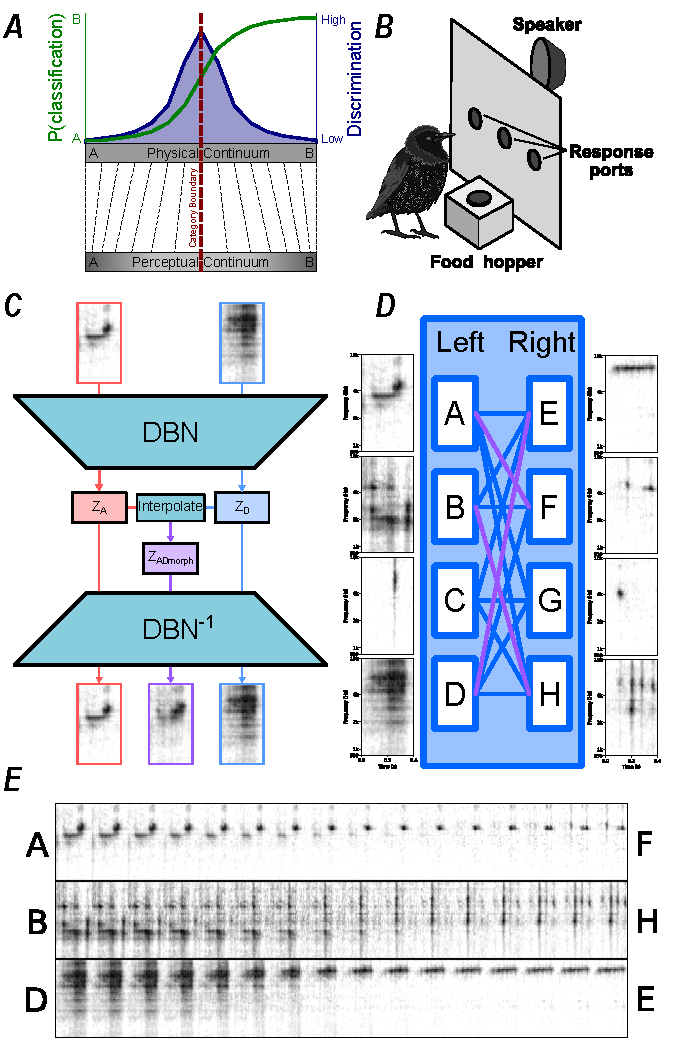
\includegraphics[width=114mm]{figures/fig01_task_outline.pdf}
  \caption[Task outline]
{(continued on following page.)
\index{outline}}
  \label{fig:outline}
\end{figure}

\begin{figure}[tp]
  \contcaption{(A) A schematic of idealized categorical perception. \emph{Top}: The lower scale depicts a series of stimuli that are spaced a fixed distance apart according to some physical measure. In a perceptual representation of these stimuli the distances between adjacent stimuli may be modified in a way that groups the stimuli into categories as shown in the upper scale. \emph{Middle:} Idealized psychometric function or identification functions to illustrated the categorical perception of the nine stimuli distributed at equal intervals along the physical continuum. This is the percent identified in the indicated category plotted against the the stimulus number along the continuum, i.e. the physical scale. \emph{Bottom:} Discrimination function representing the increased sensitivity to changes in the stimuli near the categorical boundary. This is the percent correct when discriminating between same or different stimuli pairs. This would be inversely correlated to the just noticeable distance along the continuum.
(B) A diagram of the operant behavioral apparatus which consists of response ports with IR beak detection sensors, a food hopper to provide access to a food reward, and a speaker hidden behind the panel to present auditory stimuli.
(C) A diagram of a \DBN autoencoder. A spectrogram representation of a 400 ms song motif is fed into fully connected compressive layers. The network consists of 5 hidden layers with 1024, 512, 256, 128, and 64 units each.
(D) Diagram of the behavioral task. Spectrograms of the initial 8 randomly chosen 400 ms long motifs, labeled A-H, and their reward associated responses. Once the performance on these 8 reached a sufficient stable level, interpolated morph motifs, indicated by the 16 connecting lines were probed using a ratcheting double staircase procedure to allow the birds to determine their own behavioral boundaries.The 3 example morph dimensions displayed to the left are highlighted in blue.
(E) Three example interpolated morph dimensions generated using the \DBN. 16 (of 128 used) example motifs for each morph dimension. Spectrogram representation with frequency on y-axis and time on the x-axis. Each motif is 400 ms long.}
\end{figure}